\chapter{Türerkennung}

Die Türerkennung erfolgt in mehreren Schritten. Zuerst, wird im Bild nach Liniensegmenten gesucht. Die gefundenen Segmente müssen hinsichtlich Länge und Ausrichtung optimiert werden. Anschliessend muss nach möglichen Vier-Kanten-Paaren gesucht werden, welche möglicherweise eine Tür bilden. Die gefundenen Kandidaten werden dann noch evaluiert, um den besten Treffer zu bestimmen.

\section{Kantendetektion}

Es existieren verschiedene Algorithmen um Kanten in Bildern zu suchen. In dieser Arbeit wurden speziell die "Probabilistic Hough Transform" und die "Line Segment detection using Weighted Mean-Shift" oder kurz LSWMS untersucht. Beide sind darauf spezialisiert Geraden zu finden, wobei es merkliche Unterschiede zwischen den zwei Methoden gibt.

\subsection{Probabilistic Hough Transform}

In der Literaturn wird der Term Probabalistic Hough Transform (PHT) mit verschiedenen Ideen bezüglich der Optimierung der Standard Hough Transform (SHT) assoziiert. Wir beziehen uns auf die Methode von Kiryati \cite{kiryati} welche Stichproben verwendet um die Effizienz der SHT zu verbessern.
\paragraph{}
Die Standard Hough Transform wird dazu verwendet um die Parameter von Features, wie in unserem Fall Linien, zu ermitteln. Als Ausgangspunkt wird ein Binärbild verwendet, in welchem jedes aktive Pixel (weiss) Teil einer Kante oder Linie aus dem Originalbild ist. Die SHT bildet jedes dieser Pixel auf verschiedene Punkte im Hough Raum ab, in Form eines Sinusoiden. Dieser stellt alle Linien dar welche durch diesen Pixel verlaufen könnten. Diese Abbildungsphase wird auch Voting Phase genannt. Sind mehrere aktive Pixel colinear, so werden sich ihre Sinusoiden kreuzen. Sucht man nun die Punkte im Hough Raum wo sich viele Sinusoiden kreuzen, kann man daraus die Parameter der Linien im Originalbild bestimmen.
\paragraph{}
Im Unterschied zur Standard Hough Transform verwendet die Probabalistic Hough Transform nur einen Teil, eine Stichprobe, der aktiven Pixel im Binärbild. Die PHT geht davon aus, dass ein Anteil $\alpha$ (0\% < $\alpha$ < 100\%) ausreicht um die Parameter der Linien im Bild zu ermitteln. Kiryati kam zum Ergebnis, dass ab einem bestimmten Threshold $\alpha_t$ vermehrt False-Positives bei der Detektion auftreten. Wähl man mit Hilfe einer Probability Density Function ein Subset $\alpha$ $\approx$ $\alpha_t$ so kann man den Rechenaufwand erheblich reduzieren ohne signifikante Abstriche bei der Qualität der Ergebnisse. Der Bereich von $\alpha_t$ liegt bei 5\%-15\%, je nach Anwendungsfall.

\begin{figure}[!ht]
\centering
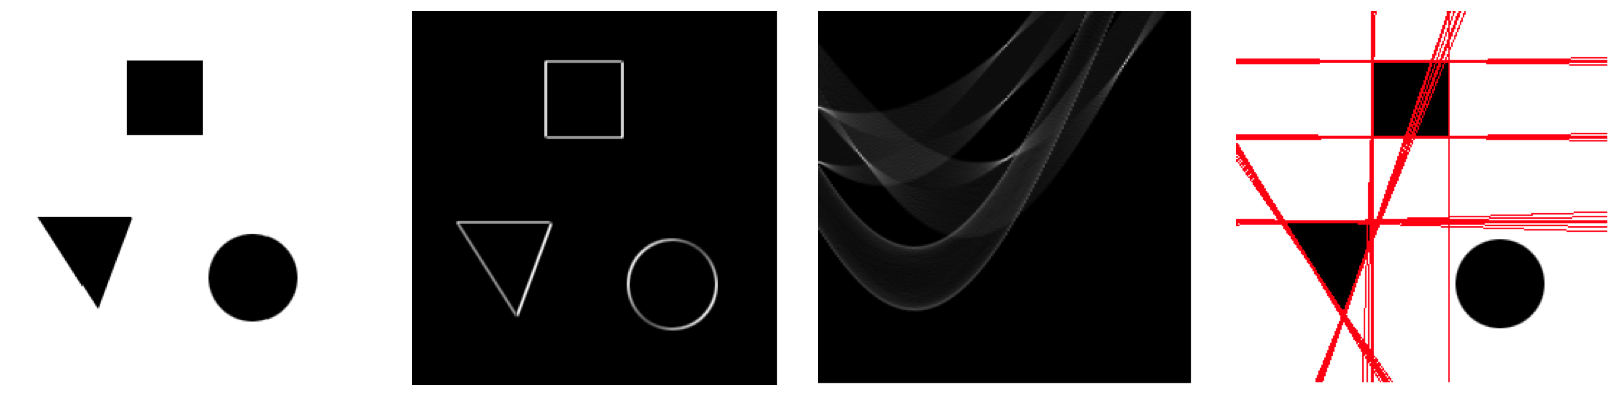
\includegraphics[scale=0.25]{images/hough-transform} 
\caption{Verarbeitungsschritte der Standard Hough Transform. Ausgangsbild, Binärbild, Hough Raum und die gefundenen Linien. Quelle \cite{kiryati}}
\label{fig:hough-transform}
\end{figure}

\pagebreak

\subsection{Line Segment detection using Weighted Mean-Shift}

\begin{figure}[!ht]
\centering
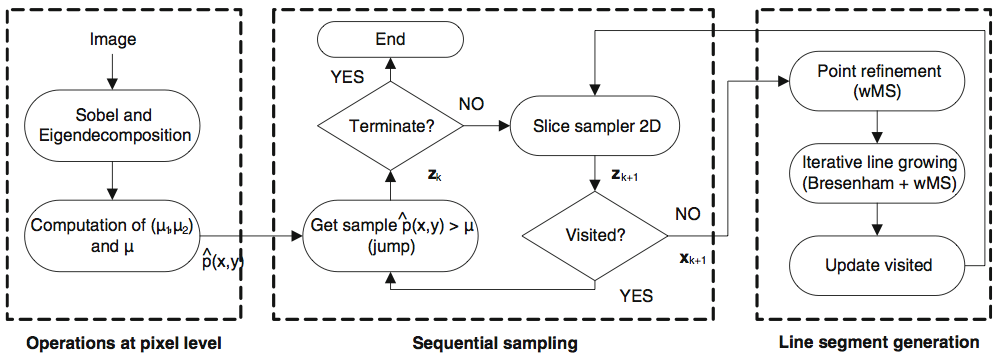
\includegraphics[width=\textwidth]{images/lswms} 
\caption{Ablaufschema des LSWMS Algorithmus. Im ersten Teil wird wie Wahrscheinlichkeitsverteilung $\hat{p}(x,y)$ anhand der Parameter $\mu_1$ und $\mu_2$ ermittelt. Im zweiten Teil wird das erste Sample generiert und der Slice-Sampling-Prozess wird gestartet, um kontinuierlich Stichproben $z_k$ zu erhalten. Im dritten und letzten Teil werden die Samples verfeinert und als Ausgangspunkte für das iterative Line-Growing verwendet, welches die gesuchten Liniensegmente liefert. Quelle \cite{nieto}}
\label{fig:lswms}
\end{figure}
\noindent
Abb. \ref{fig:lswms} veranschaulicht den Ablauf des "Line Segment detection using Weighted Mean-Shift" (LSWMS) Algorithmus. Im ersten Teil wird die Wahrscheinlichkeitsverteilung für jedes Pixel von Bild $I$ berechnet, so dass $\hat{p}(x, y)$ angibt, wie wahrscheinlich es ist, dass das Pixel $(x, y$) Teil eines Liniensegmentes ist. Diese Wahrscheinlichkeitsverteilung, parametrisiert durch $\mu_1$ und $\mu_2$, wird anhand der Tensor Matrix und den dazugehörigen Eigenvalues errechnet. Gute Kandidatenpixel müssen zwei Bedingungen erfüllen. Zum einen muss der Betrag des Gradienten auf eine gewisse Signifikanz des Pixels hindeuten und zum anderen muss eine dominante Gradienten-Richtung in der Nachbarschaft des Pixels vorhanden sein.
\paragraph{}
Der zweite Teil "sequential sampling" selektiert, basierend auf $\hat{p}(x,y)$, kontinuierlich Pixel ($z_k$) welche eine hohe Wahrscheinlichkeit besitzen zu einem Liniensegment zu gehören. Gleichzeitig wirk sichergestellt, dass kein Pixel eines Segmentes mehrmals gesampelt wird. Dies ist ein wichtiger unterschied zu PHT, da es die Effizienz von LSWMS im Vergleich zu PHT erhöht. Der Slice Sampler basiert auf dem Markov-Chain-Monte-Carlo-Verfahren\footnote{\protect\url{http://de.wikipedia.org/wiki/MCMC-Verfahren}}, welches es erlaubt kontinuierlich Stichproben aus einer bestimten Wahrscheinlichkeitsverteilung $p$ zu ziehen, welche in unserem Fall die Qualität des Kandidatenpixel angibt.
\paragraph{}
Die Wahrscheinlichkeitsverteilung wird beim LSWMS Algorithmus anhand der Eigenvalues $(\lambda_1, \lambda_2)$ eines jeden Pixel berechnet. Wobei $f$ die Eigenvalues $(\lambda_1, \lambda_2)$ zu einem beliebigen Pixel $(x, y)$ zurückgibt.

\begin{equation}
\begin{split}
p = g \circ f:  &I \to (\lambda_1, \lambda_2) \to \mathbb{R} \\
                &(x, y) \mapsto \hat{p}(x, y) = g(f(x, y))
\end{split}
\end{equation}
\noindent
Die Funktion erfüllt zwei wichtige Kriterien. Zum einen gibt sie nur hohe Werte zurück für Eigenvalues-Paare bei dem ein Wert deutlich grösser ist als der Andere. Zum anderen fällt der Wert rapide ab, wenn beide Werte hoch oder tief sind. $g$ gibt die Wahrscheinlichkeit an, dass ein Eigenvalue-Paar zu einem Liniensegment gehört.

\begin{equation}
g(\lambda_1, \lambda_2) = (1 - exp(-\lambda_1/\mu_1)) exp(-\lambda_2/\mu_2)
\end{equation}
\noindent
$\mu_1$ und $\mu_2$ sind die Durchschnittswerte aller Eigenvalues über das ganze Bild. Diese wurden im ersten Teil ermittelt. Stellt man die Verteilung visuell dar, so ergibt sich das Bild in Abb. \ref{fig:lswms-eigenvalues}.

\begin{figure}[!ht]
\centering
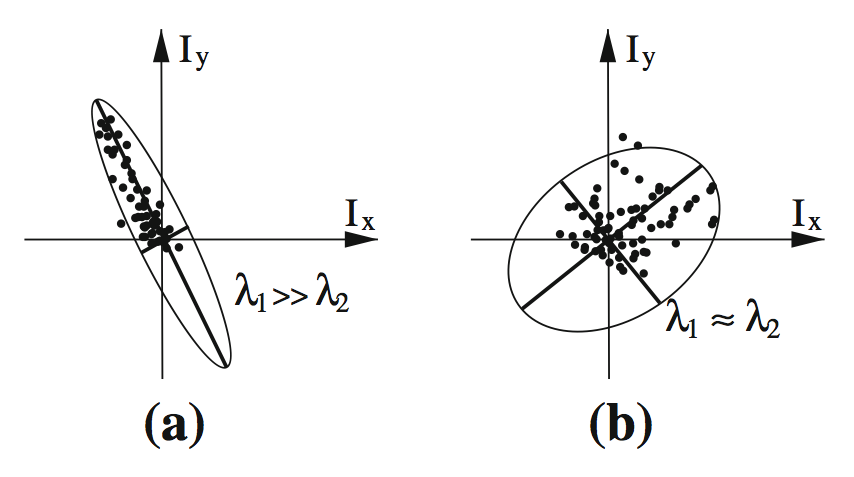
\includegraphics[width=\textwidth]{images/lswms-eigenvalues} 
\caption{Eigenvalues welche die Gradientenstruktur abbilden. Die schwarzen Punkte sind die Werte der Nachbarpixel eines Pixels $(I_x, I_y)$. a) Verteilung eines Liniensegmentes. b) Verteilung einer Ecke oder einer heterogenen Gradienten. Quelle \cite{nieto}}
\label{fig:lswms-eigenvalues}
\end{figure}
\noindent
\paragraph{}
Basierend auf diesen Grundlagen werden die Liniensegmente wie folgt ermittelt. Initial wird iterativ ein erster Kandidatenpixel gesucht, welcher die Bedingung $\hat{p}(x, y) > \mu$ erfüllt. $\mu$ ist der Mittelwert von $\hat{p}(x, y)$ über das ganze Bild. Dies stellt sicher, das für den Schritt der Segmentgenerierung eine optimale Ausgangslage geschaffen wird. So gibt es so wenig Fehlversuche wie möglich. Nachfolgend such der Sampler Pixel mit einem ähnlichen Wert für $\hat{p}(x, y)$ wie der Initialpixel. Jedes mal wenn ein Liniensegment generiert wird, werden sämtliche Pixel des Segmentes aus dem Pool der Pixel aus dem der Sampler wählt entfernt. Auch, werden die Nachbarpixel innerhalb einer definierten Fensters von $r x r$ entfernt, wobei r die räumliche Weite des Mean Shift ist. Aufgrund dieser Tatsache kann der Fall eintreten, dass der Slice Sampler feststellt, dass alle Pixel in der Nachbarschaft des initialen Pixels bereits verarbeitet wurden. In diesem Fall wird ein neuer Initialpixel gesucht, welcher die gegebenen Kriterien erfüllt. Der Sampler sucht so lange nach neuen Kandidaten bis keine geeigneten mehr gefunden werden oder bis eine gegebene Obergrenze bei der Anzahl zu suchender Liniensegmente erreicht wurde.
\paragraph{}
Die geeigneten Bildpunkte welche vom Slice Sampler ermittelt werden, werden kontinuierlich dem Line Segment Generator übergeben. Erhält dieser ein Sample $z_k$ und die dazugehörige Orientierung der Nromalen $\theta_k$, so steuert er die Richtung des Generierungsprozesses anhand des Vektors $\textbf{x}_{k} = (x_k, y_k, \theta_k)$. Obwohl der Sampler bereits sehr gute Kandidaten liefert, besteht immer noch die Möglichkeit, dass in der Nachbarschaft von $\textbf{x}_k$ ein Bildpunkt mit einem höheren Wert für $\hat{p}(x, y)$ vorhanden ist. Aus diesem grund wird mittels Weighted Mean Shift (wMS) nach einem Optimum $\hat{\textbf{x}}_k$ gesucht. Mean Shift (MS) ist ein iterativer, parameterfreier Algorithmus, welcher dazu eingesetzt werden kann lokale Maxima einer unbekannten Dichtefunktion zu ermitteln, wenn eine Menge von Samples vorhanden ist. Bei jeder Iteration startet MS bei einer initialen Stichprobe und bewegt sich in richtung der dichtesten Region innerhalb des Suchraumes. LSWMS gewichtet die Stichproben zusätzlich noch anhand der zuvor berechneten Wahrscheinlichkeiten $\hat{p}$.
\paragraph{}
Anhand des verfeinerten Punktes $\hat{\textbf{x}}_k = (\hat{x}_k, \hat{y}_k, \hat{\theta}_k)$ wird dann die Generierung des Segmentes vorgenommen, basierend auf dem Bresenham Algorithmus \cite{bresenham}. Das obere Segment in der Abb. \ref{fig:lswms-line-growing}a veranschaulicht diesen Vorgang.

\begin{figure}[!ht]
\centering
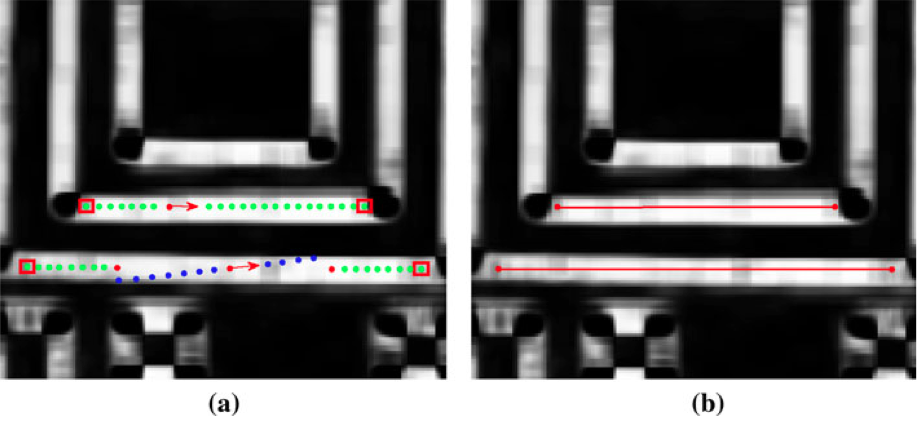
\includegraphics[width=\textwidth]{images/lswms-line-growing} 
\caption{Oriented Line Growing. a) Oberes Segment mit einer genauen Wachstumsrichtung. Unteres segment mit einem Wachstumsprozess welcher eine Verfeinerung der Richtung benötigt. b) In beiden Fällen wurde ein korrektes Segment ermittelt, welches sich innerhalb des Gradienten der Kante befindet. Quelle \cite{nieto}}
\label{fig:lswms-line-growing}
\end{figure}

\subsection{Evaluation}

Die Entscheidung fiel auf den LSWMS Algorithmus, aus mehreren Gründen. LSWMS wurde von Anfang an für die unbeaufsichtigte Kantendetektion innerhalb von Echtzeitanwendungen konzipiert. Da die Umgebungen in denen die Türdetektion stattfindet stark variieren können, ist es nicht möglich im vorhinein fixe Parameter für die Hough-Transformation zu definieren, welche überall gleich gut funktionieren. LSWMS bietet im Schnitt unter sich verändernden Verhältnissen die bessere Leistung. Der Algorithmus erforder zwar auch einen Parameter r, welcher oben erklärt wurde, jedoch kann dieser auf dem Standardwert 3 belassen werden. Mit diesem gibt LSWMS akzeptable Resultate zurück.
\paragraph{}
Ein weiterer Faktor ist die Qualutät der zurückgegebenen Resultate. Die Anzahl fehlerhaft erkannten Kanten ist bei Hough erheblich höher als bei LSWMS und wirkt sich damit auch auf die Performance der weiteren Verarbeitungsschritte negativ aus. Die Möglichkeit bei LSWMS eine Obergrenze bezüglich der Anzahl erwarteter Treffer angeben zu können war ebenfalls ausschlaggebend. Bei "ruhigen" Bildern mit wenig potentiellen Kanten wirkt sich dies wenig aus. Bilder welche z.B. Türem mit Holzmuster enthalten führen bei Hough zu einer Fehlerquote von teilweise über 50\%.
\paragraph{}
Der letzte Faktor welcher zur Entscheidung geführt hat LSWMS vorzuziehen war die Gesamtperformance. Hough benötigt als Input ein Kantenbild, welches zuvor mit einem separaten Algorithmus aufgearbeitet werden muss, z.B. Canny\footnote{\protect\url{http://de.wikipedia.org/wiki/Canny-Algorithmus}}. Dieser Schritt führt zusätzliche Parameter ein, welche situationsbedingt optimiert werden müssen und erhöht die Verarbeitungszeit der Hough-Transformation. Da Canny empfindlich gegenüber Rauschen im Bildmaterial ist, muss ein weiterer Verarbeitungsschritt vorangestellt werden. Bevor Canny angewendet wird, werden mittels einem Gausschen Filter Störfaktoren reduziert. Um ein optimales Ergebnis zu erhalten müssen vertikale und horizontale Kanten separat gesucht werden. Dies hat zu folge das die Hough-Transformation zweimal dürchgeführt werden muss (Canny muss nur einmal angewendet werden, beide Male kann das selbe Kantenbild verwendet werden).
\paragraph{}
Für den Vergleich der Hough-Transformation und LSWMS wurden folgende Parameter verwendet:
\paragraph{}
Gauss Filter (medianBlur)\footnote{\protect\url{http://docs.opencv.org/modules/imgproc/doc/filtering.html?highlight=medianblur#medianblur}}
\begin{itemize}
	\item kSize: 5
\end{itemize}
Canny Edge Detection\footnote{\protect\url{http://docs.opencv.org/doc/tutorials/imgproc/imgtrans/canny_detector/canny_detector.html}}
\begin{itemize}
	\item lowThreshold: 20
	\item highThreshold: 80
	\item kernelSize: 3
\end{itemize}
Probabilistic Hough Transform\footnote{\protect\url{http://docs.opencv.org/doc/tutorials/imgproc/imgtrans/hough_lines/hough_lines.html}}
\begin{itemize}
	\item rho: 1
	\item theta: 1 rad
	\item threshold: 80
	\item minLinLength: 30
	\item maxLineGap: 10
\end{itemize}
LSWMS
\begin{itemize}
	\item numMaxLSegs: 1000
\end{itemize}
\noindent
Die gelben Linien stellen die gefundenen Kanten bzw. Kanstensegmente dar.
\pagebreak

\begin{figure}
\subfloat[Ergebnis Hough-Transformation]{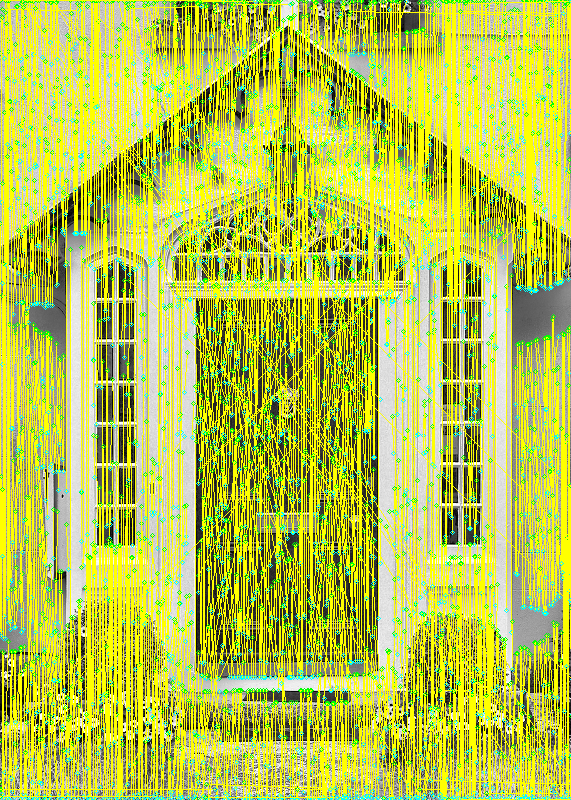
\includegraphics[width=0.47\textwidth]{images/hough-raw-segments}}\qquad
\subfloat[Ergebnis LSWMS]{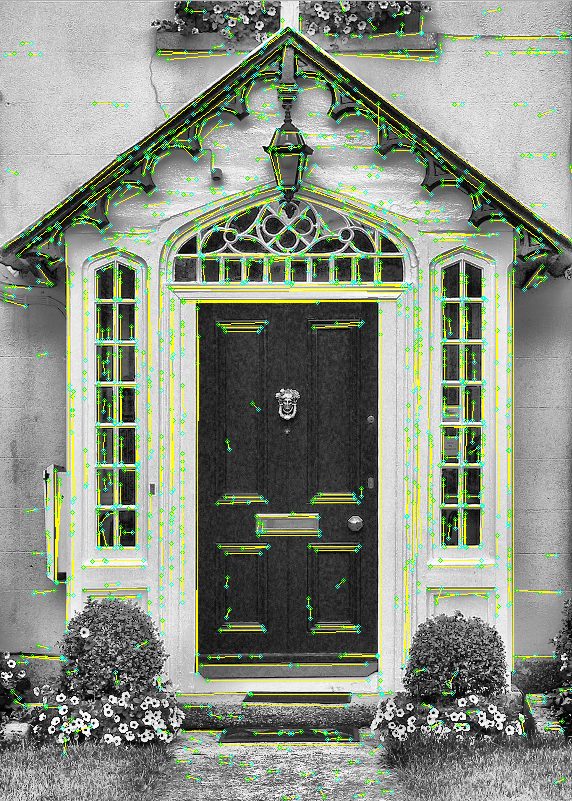
\includegraphics[width=0.47\textwidth]{images/lswms-raw-segments}}
\caption{Vergleich PHT und LSWMS}
\label{fig:comp-pht-lswms}
\end{figure}
\noindent
Dies ist nur ein Bild von zehn getesteten. Die Bilder welche während der Entwicklung zum Testen verwendet wurden können im Projektverzeichnis unter Data/Images/Doors/Misc gefunden werden. Es ist klar ersichtlich, dass LSWMS das qualitativ bessere Ergebnis liefert. Einziger Nachteil hier ist, dass LSWMS oft nicht durgehende Kanten erkennt sondern kleinere Segmente entlang der Kante zurückgibt. Neben der Qualität der Resultate wurde auch die Performance beider Methoden analysiert. Da einige Testbilder grösser sind als in der finalen Applikation benötigt, wurden alle Bilder auf eine Höhe von 800 Pixel verkleinert. Nachfolgend das Ergebnis (Durchschnitt aus 100 Durchgängen):

\begin{itemize}
	\item Hough: 165ms, 1871 Segmente
	\item LSWMS: 64ms, 868 Segmente
\end{itemize}
\noindent
Auch hier ist LSWMS Hough überlegen. Obwohl LSWMS für Echtzeitanwendungen konzipiert wurde, kann mit den gemessenen 64ms Verarbeitungszeit pro Frame kein flüssiges Videobild bei 28fps wiedergegeben werden.

\section{Implementation}

\begin{figure}[!ht]
\centering
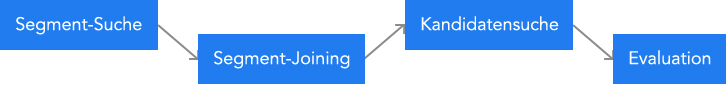
\includegraphics[width=\textwidth]{images/door-detection} 
\caption{Ablauf der Türerkennung}
\label{fig:door-detection}
\end{figure}
\noindent
Wie bereits zu beginn des Kapitels erwähnt, besteht der Prozess der Türerkennung aus mehreren Teilschritten (Abb. \ref{fig:door-detection}). Als erstes wird der LSWMS Algorithmus angewendet. Dieser Arbeitet auf Graustufenbildern. Somit wird der Input entsprechend konvertiert. Da die Lichtverhältnisse vor allem and den Türkanten oft subobtimal sind, aufgrund eines leichten Schattenwurfes, wird eine Contrast Limited Adaptive Histogram Equialization (CLAHE) angewendet mit einem Clip Limit von 5 und einer Fenstergrösse von 8. Diese Werte wurden experimentel ermittelt. Der Grund, dass CLAHE angewendet wurde und keine normale (Adaptive) Histogram Equalization ist, dass festgestellt wurde, dass die Verstärkung von Rauschen und von feinen Muster (z.B. Holzmaserungen) die Qualität der Resultate von LSWMS verringert. Weiterhin ist es wichtig, dass die Regionen um die Tür herum ausgebessert werden. Dies ist damit gegeben, dass CLAHE den Kontrast immer innerhalb eines bestimmten Fensters ausgleicht. Um sichtbare Kanten der einzelnen Fenster zu vermeiden, wird die Randregion noch interpoliert. Der Unterschied der globalen Histogram Equalization und CLAHE wird in Abb. \ref{fig:clahe} verdeutlicht. Ein Beispiel wie die Ausgabe der LSWMS Erkennung aussieht, ist in Abb. \ref{fig:lswms-output} ersichtlich.

\begin{figure}
\subfloat[Ausgangsbild]{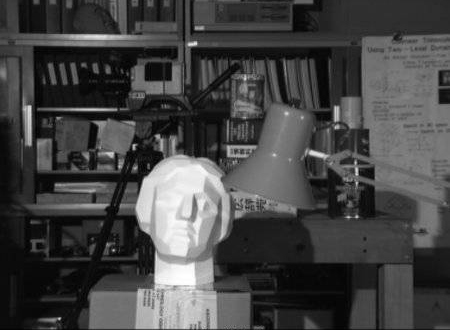
\includegraphics[width=0.47\textwidth]{images/clahe-orig}}\qquad
\subfloat[Global Histogram Equalization]{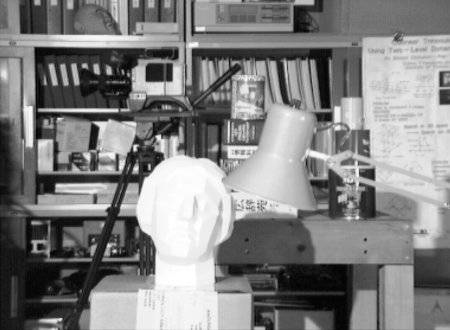
\includegraphics[width=0.47\textwidth]{images/clahe-ghe}}\qquad
\subfloat[Contrast Limited Adaptive Histogram Equialization]{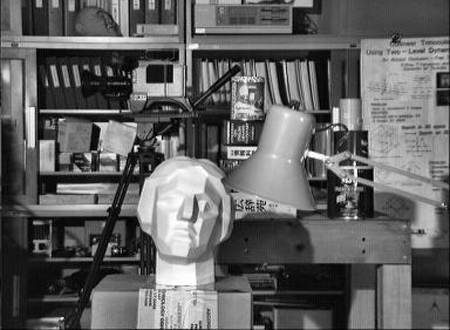
\includegraphics[width=0.47\textwidth]{images/clahe}}\qquad
\caption{Vergleich Global Histogram Equalization und CLAHE}
\label{fig:clahe}
\end{figure}

\begin{figure}
	\subfloat[Segmente wie sie von LSWMS gefunden werden]{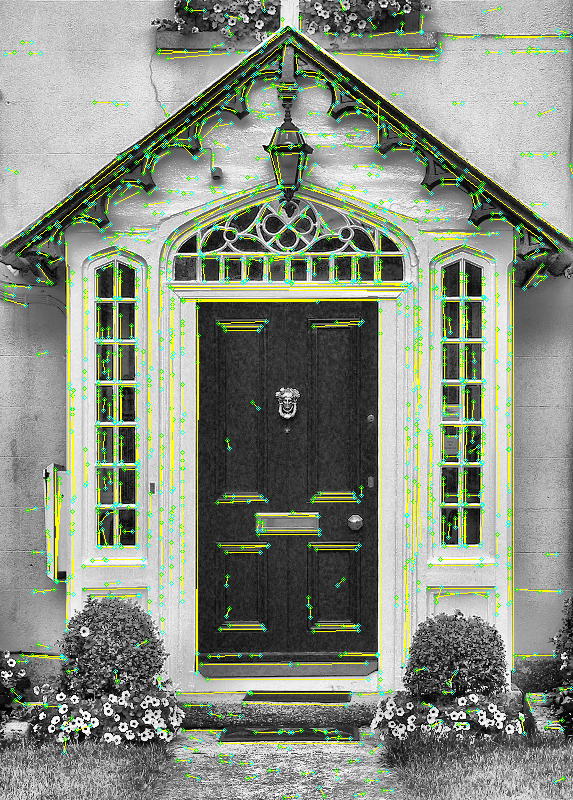
\includegraphics[width=0.45\textwidth]{images/seg-raw}\label{fig:lswms-output}}\qquad	
	\subfloat[Segmente kategorisiert in horizontal (Rot) und vertikal (Gelb)]{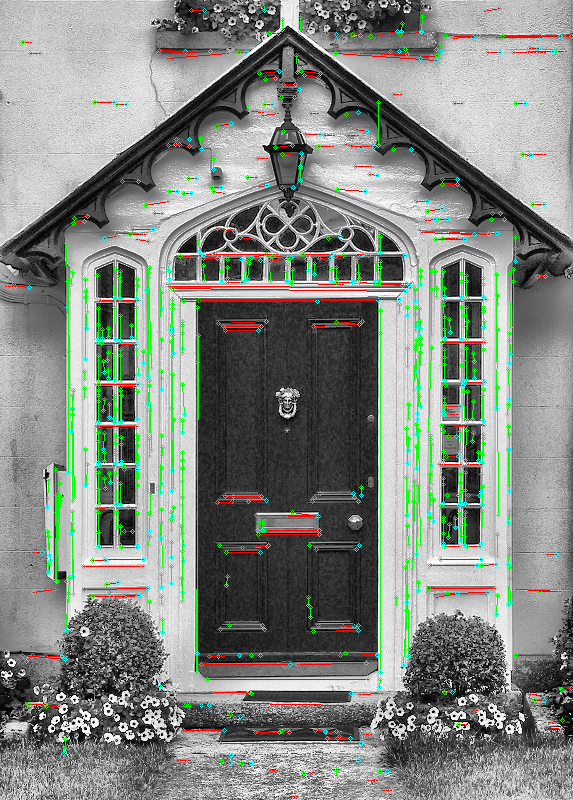
\includegraphics[width=0.45\textwidth]{images/seg-categorized}\label{fig:segs-categorized}}\qquad	
	\subfloat[Verschmolzene Segmente]{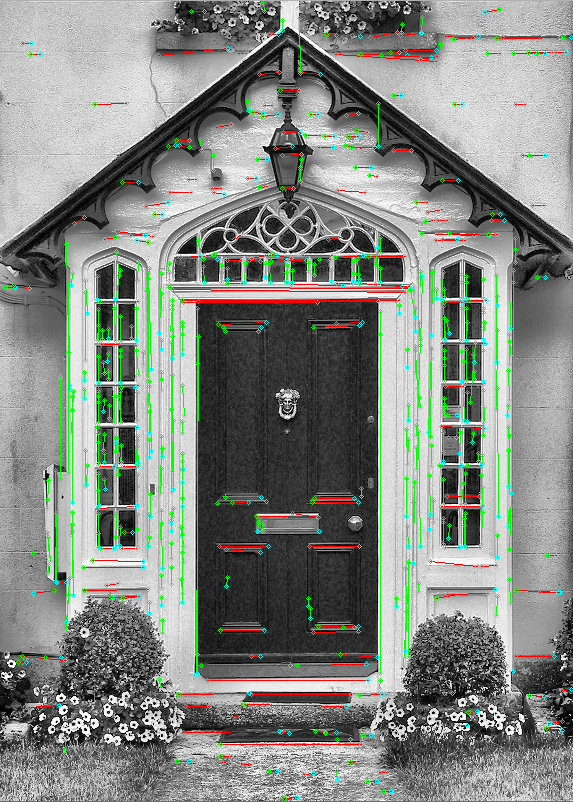
\includegraphics[width=0.45\textwidth]{images/seg-joined}}	\qquad	
	\subfloat[Verlängerte Segmente]{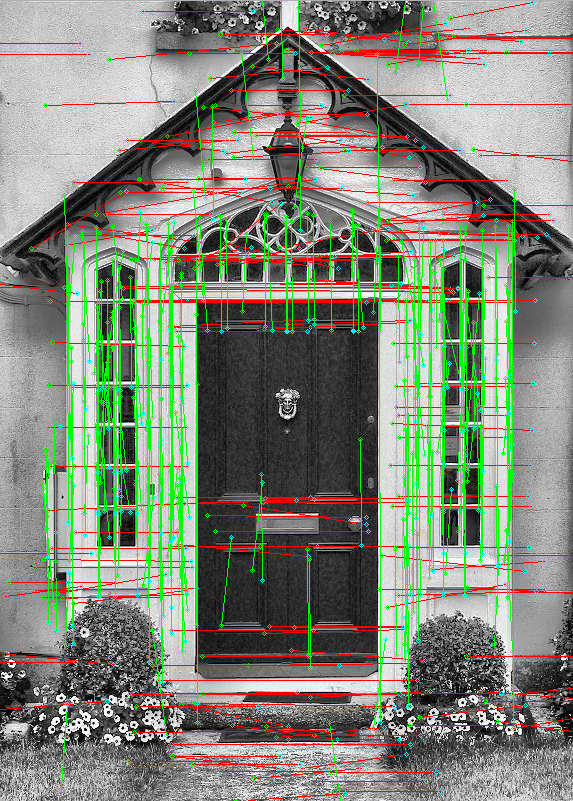
\includegraphics[width=0.45\textwidth]{images/seg-grow}}	
	\caption{Verarbeitungsprozess Türerkennung}
\end{figure}

\begin{figure}
	\ContinuedFloat
	\centering		
	\subfloat[Gefundene Kandidaten]{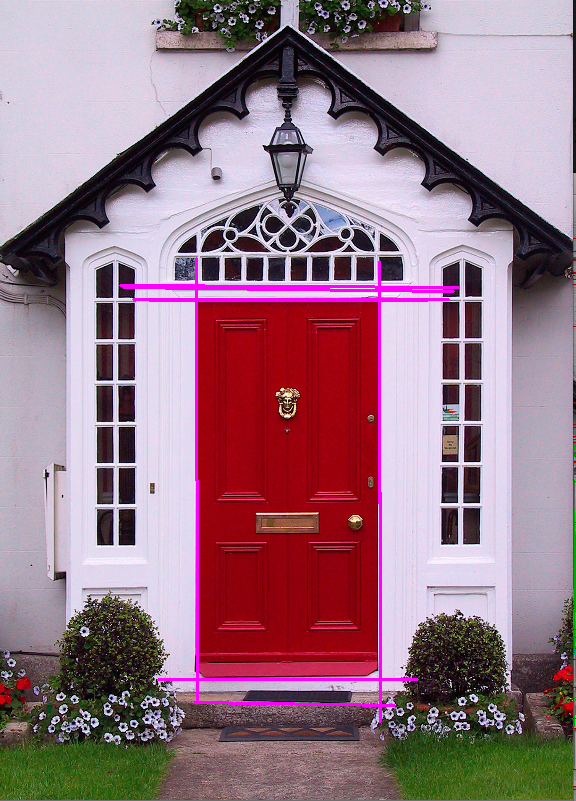
\includegraphics[width=0.45\textwidth]{images/seg-candidates}}\qquad
	\subfloat[Erkannte Tür]{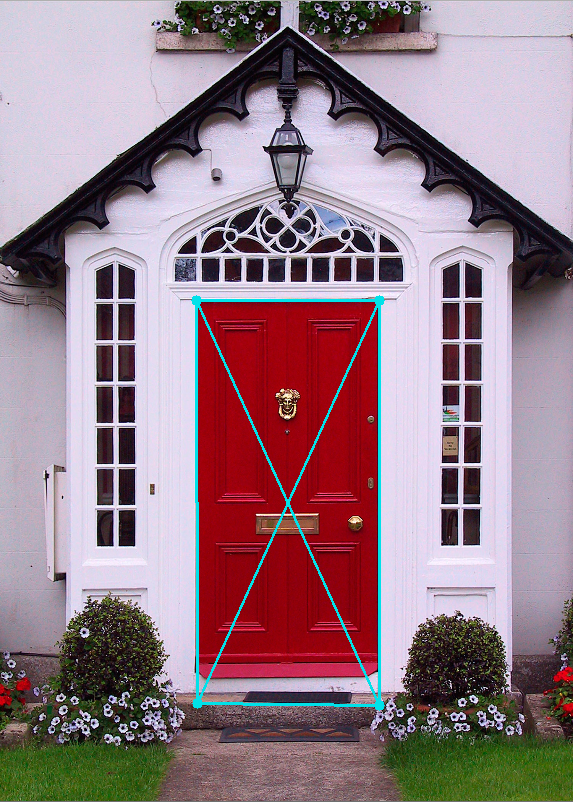
\includegraphics[width=0.45\textwidth]{images/seg-detected}}\qquad
	\caption{Verarbeitungsprozess Türerkennung}
	\label{fig:door-detection}
\end{figure}

\subsection{Kategorisierung}
Im nächsten Schritt werden die gefundenen Liniensegmente nach ihrer Ausrichtung kategorisiert (Abb. \ref{fig:segs-categorized}). Hierzu muss zuerst bestimmt weren, was horizontal und vertikal ist. Wird die Türe frontal aufgenommen, so sind dies die gewohnten werde $0$ für horizontal und $\frac{\pi}{2}$ für vertikal. Nimmt man die Türe seitlich auf, so werden vor allem die Horizontale verzerrt. Um nun zu bestimmen welcher Winkel die als Ausgangspunkt für die Horizontale ist, werden bestimmte Annahmen getroffen. Horizontale Linien weichen auch bei einer starken seitlichen aufnahme nie mehr als 50° (0.839rad) von der unverzerten Horizontale ab. Für die Vertikale wurde ein Wert von 20° (0.3491rad) festgelegt. Diese Werte wurden aus Probeaufnahmen aus verschiedenen Winkeln ermittelt und sind in Source/Ardoor/DoorDetection/DoorDetector.hpp in den Konstanten MAX\_HORIZONTAL\_DIVERGENCE bzw. MAX\_VERTICAL\_DIVERGENCE festgehalten. Da nur längere Segmente verlässliche Informationen bezüglich der Ausrichtung liefern, wird eine Mindestlänge von 10\% der Diagonalen vorrausgesetzt. Alle Längenangaben bei der Türerkennung sind anhand prozentualer Anteile gegenüber der Diagonalen festgelegt, da die Diagonale die längst-mögliche Strecke in jedem Bild ist. So sind die Vorraussetzungen für jede Bildgrösse die selben. Wurden die Grenzwerte ermittelt, werden die Segmente nun kategorisiert. Hier wird eine Abweichung von 15° (MAX\_GRADIENT in Source/Ardoor/DoorDetection/LineSegment.hpp) zur Vertikalen bzw. Horizontalen erlaubt, um Fehler bei der Liniensegment-Erkennung auszugleichen und um eine bessere Grundlage für den nächsten Verarbeitungsschritt zu schaffen.

\subsection{Segment Joining}
Da die gefundenen Kanten oft nicht aus durchgehenden Segmenten bestehen sondern aus mehreren kleinen (Abb. \ref{fig:segments-pre-join}), müssen in diesem Schritt Liniensegmente die nahe bei einander liegen und eine änhliche Ausrichtung haben verschmolzen werden. Dabei wird wie folgt vorgegenagen. Als erstes wird die Distanz der Segmente berechnet. Dabei müssen mehrere Fälle unterschieden werden.

\begin{itemize}
	\item Segmente sind Parallel $\Rightarrow$ Die Distanz kann von jedem Punkt aus in der "Überlappungszone" bestimmt werden kann.
	\item Segmente stehen schief zueinander $\Rightarrow$ Die Segmentpunkte mit der geringsten Distanz müssen ermittelt werden.
	\item Segmente haben keine "Überlappungszone" $\Rightarrow$ Distanz von End- zu Startpunkt wird berechnet
	\item Segmente kreuzen sich $\Rightarrow$ Schnittpunkt muss ermittelt werden
\end{itemize}

\begin{figure}[!ht]
\centering
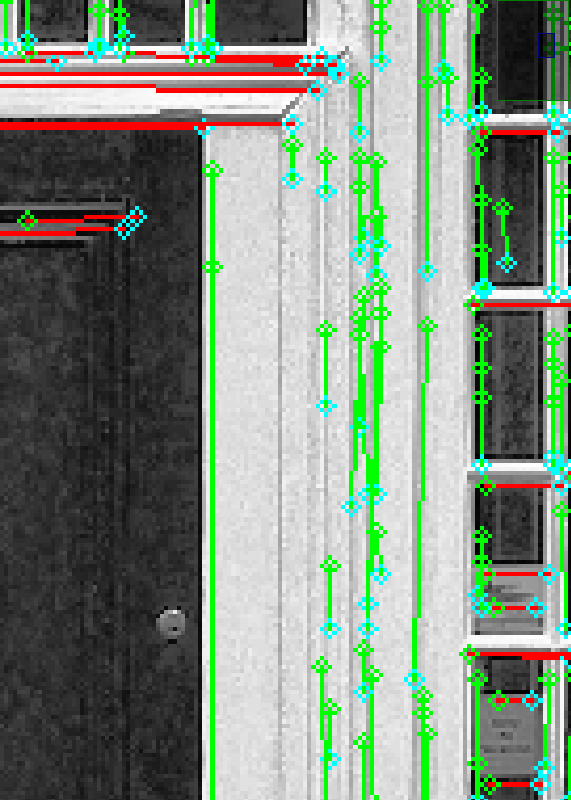
\includegraphics[width=0.5\textwidth]{images/segments-pre-join} 
\caption{Segmente vor der Verschmelzung (gezoomt)}
\label{fig:segments-pre-join}
\end{figure}
\noindent
Eine Distanz von max. 8px hat sich als guter Wert erwiesen. Wurden zwei Segmente gefunden die nahe genug bei einander sind, wird das Segment Joining initialisiert. Hier wird zuerst überprüft, ob es Sinn macht die Segmente zu vereinen. Liegt ein Segment innerhalb des Bereiches des anderen, so macht dies keinen Sinn, da das Segment nicht erweiter wird (Abb. \ref{fig:segment-joining-1}).

\begin{figure}[!ht]
\centering
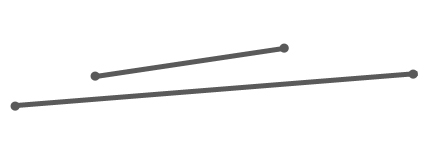
\includegraphics[width=0.5\textwidth]{images/segment-joining-1} 
\caption{Hier macht es keinen Sinn die zwei Segmente zu verschmelzen}
\label{fig:segment-joining-1}
\end{figure}
\noindent
Ist dies nicht der Fall, so wird ermittelt, welches Segment die bessere Ausrichtung gegenüber der errechneten Horizontalen bzw. Vertikalen hat. Die bessere Ausrichtung wird beim Verbinden beibehalten. Anschliessend werden die Längen addiert und das neue Segment wird zwischen den zwei Ausgangssegmenten platziert (Abb. \ref{fig:segment-joining-2}).

\begin{figure}[!ht]
\centering
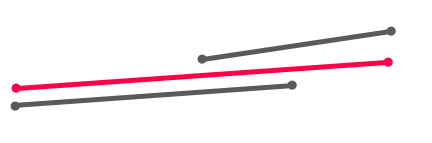
\includegraphics[width=0.5\textwidth]{images/segment-joining-2} 
\caption{Ausgangssegmente grau und verschmolzenes Segment rot}
\label{fig:segment-joining-2}
\end{figure}

\subsection{Kandidatensuche}

\subsection{Performance}

\subsection{Verbesserungsmöglichkeit}